\documentclass{standalone}
\usepackage{tikz}
\usepackage{xcolor}
\begin{document}
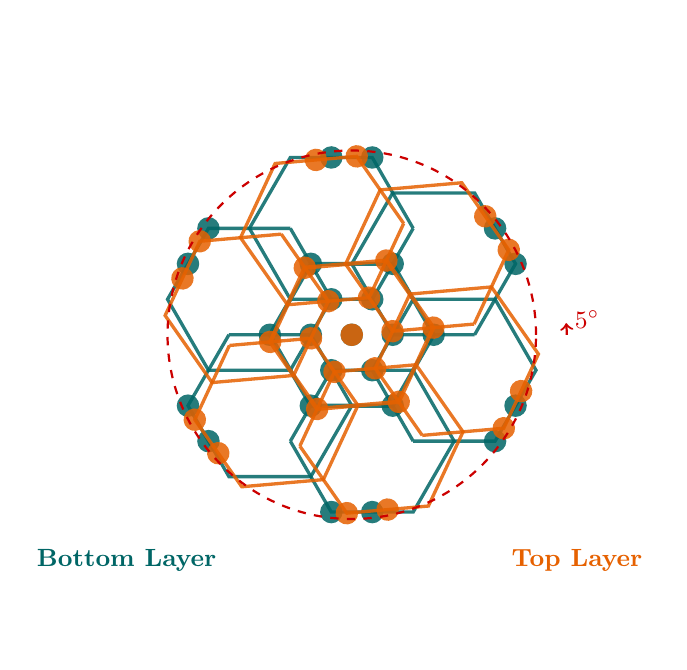
\begin{tikzpicture}[scale=1.3]
    % Define improved custom colors
    \definecolor{bottomlayer}{RGB}{0,102,102}
    \definecolor{toplayer}{RGB}{230,97,0}
    
    % Parameters
    \def\r{0.8}        % radius of hexagons
    \def\theta{5}      % twist angle
    \def\atomsize{0.11} % atom size
    
    % Function to draw a hexagonal lattice layer
    \newcommand{\hexlayer}[2]{ % parameters: rotation, color
        \begin{scope}[rotate=#1]
            % Center hexagon
            \draw[#2, line width=1.5pt] 
                (0:\r) -- (60:\r) -- (120:\r) -- (180:\r) -- (240:\r) -- (300:\r) -- cycle;
            
            % Surrounding hexagons - first ring
            \foreach \a in {0,60,...,300} {
                \pgfmathsetmacro\cx{1.5*\r*cos(\a)}
                \pgfmathsetmacro\cy{1.5*\r*sin(\a)}
                
                \draw[#2, line width=1.2pt] 
                    (\cx,\cy) -- ++(60+\a:\r) -- ++(120+\a:\r) -- ++(180+\a:\r)
                    -- ++(240+\a:\r) -- ++(300+\a:\r) -- ++(0+\a:\r);
            }
            
            % Atoms at vertices - central hexagon
            \foreach \a in {0,60,...,300} {
                \fill[#2] (\a:\r) circle (\atomsize);
            }
            
            % Central atom
            \fill[#2] (0,0) circle (\atomsize);
            
            % Atoms at vertices - surrounding hexagons (fewer for clarity)
            \foreach \a in {0,60,...,300} {
                \pgfmathsetmacro\cx{1.5*\r*cos(\a)}
                \pgfmathsetmacro\cy{1.5*\r*sin(\a)}
                
                \foreach \b in {60,180,300} {
                    \fill[#2] (\cx,\cy) ++(\a+\b:\r) circle (\atomsize);
                }
            }
        \end{scope}
    }
    
    % Fill background
    \fill[white] (-3,-3) rectangle (3,3);
    
    % Draw bottom layer (slightly transparent for better visualization)
    \begin{scope}[opacity=0.85]
        \hexlayer{0}{bottomlayer}
    \end{scope}
    
    % Draw top twisted layer
    \begin{scope}[opacity=0.85]
        \hexlayer{\theta}{toplayer}
    \end{scope}
    
    % Draw a highlight circle to emphasize the twist region
    \draw[dashed, thick, red!80!black] (0,0) circle (1.8);
    
    % Twist angle arrow
    \draw[->, thick, red!80!black] (2.1,0) arc[start angle=0, end angle=\theta, radius=1.3];
    \node[red!80!black, font=\small\bfseries] at (2.3,0.15) {$\theta^\circ$};
    
    % Layer labels
    \node[font=\small\bfseries, bottomlayer] at (-2.2,-2.2) {Bottom Layer};
    \node[font=\small\bfseries, toplayer] at (2.2,-2.2) {Top Layer};
    
\end{tikzpicture}

\end{document}
